\documentclass[12pt,a4paper]{article}
\usepackage[margin=24mm]{geometry}
\usepackage{fontspec}
\setmainfont{Liberation Serif}
\usepackage{amsmath,amssymb,amsthm,mathtools,booktabs}
\usepackage{graphicx,caption}
\usepackage{float}
\graphicspath{{figures/}{output/figures/}}
\captionsetup{font=small,labelfont=bf}
\usepackage{unicode-math}
\setmathfont{Latin Modern Math}
\usepackage{microtype}
\usepackage[hidelinks]{hyperref}
\usepackage{enumitem}
\setlength{\parskip}{3pt}
\setlength{\emergencystretch}{2em}
\setlength{\abovedisplayskip}{8pt plus 2pt minus 2pt}
\setlength{\belowdisplayskip}{8pt plus 2pt minus 2pt}
\newtheorem{theorem}{Theorem}
\newtheorem{proposition}[theorem]{Proposition}
\newtheorem{lemma}[theorem]{Lemma}
\newtheorem{corollary}[theorem]{Corollary}
\newcommand{\R}{\mathbb R}
\newcommand{\F}{\mathbb F_2}
\newcommand{\Z}{\mathbb Z}
\newcommand{\rank}{\operatorname{rank}}
\newcommand{\Var}{\operatorname{Var}}
\newcommand{\ee}{\mathrm e}
\newcommand{\pos}[1]{(#1)_+}
\title{A $1.30^d$ Lower Bound for the Chromatic Number\ of Euclidean Space}
\author{Ilya Hoffman\\[3pt]
\normalsize\href{mailto:ilya.hoffman@gmail.com}{ilya.hoffman@gmail.com}\\[2pt]
\small\href{https://orcid.org/0009-0008-9083-2105}{https://orcid.org/0009-0008-9083-2105}}
\date{}
\hypersetup{pdftitle={A 1.30\string^d Lower Bound for the Chromatic Number of Euclidean Space},pdfauthor={Ilya Hoffman}}
\begin{document}
\maketitle
\vspace{-1.5em}
\begin{abstract}
We prove that $\chi(\R^d)\ge cC_*^d$ for an absolute constant $c>0$ and all sufficiently large $d$, where $1.309251<C_*<1.309252$. In particular, $\chi(\R^d)\ge1.30^d$ for all sufficiently large $d$. For infinitely many dimensions, the same construction gives $\chi(\R^d)\ge1.316^d$. The construction uses all integer points with six or seven allowed coordinate values on a sphere centred at $(1/4,\ldots,1/4)$. The half-integer lattice containing their midpoints gives an elementary bound on their distances. A binary matrix has an identity principal submatrix on every colour class. Newton interpolation bounds its rank by a weighted sum of coefficients of a power of an explicit polynomial. One elementary binomial estimate supplies matching inverse-square-root factors in the vertex count and the rank bound, leaving a constant prefactor. Four concave lower bounds cover the interval forced by the choice of a power of two. The rounded bound also has a short proof using four integer comparisons with a common frequency denominator of $200$. The algebraic arguments and all finite arithmetic data are included in the paper.
\end{abstract}
\noindent\textit{2020 Mathematics Subject Classification.} Primary 05C15; Secondary 52C10, 15A03.

\section{The result and the proof}
The chromatic number $\chi(\R^d)$ is the least number of colours needed to colour $\R^d$ so that points at distance one receive different colours.

\begin{theorem}\label{main}
There exist absolute constants $c>0$ and $d_0$ such that
\begin{equation}\label{mainbound}
\chi(\R^d)\ge cC_*^d\qquad(d\ge d_0),
\end{equation}
where $C_*$ is defined by \eqref{crossing} and satisfies
$1.309251<C_*<1.309252$. In particular, $\chi(\R^d)\ge1.30^d$ for all sufficiently large $d$.
\end{theorem}

Raigorodskii's lower exponential base $1.239\ldots$ \cite{rai} is recorded in the 2025 survey \cite[Section 1.5]{survey}. Theorem~\ref{main} concerns the same ordinary chromatic number and one forbidden Euclidean distance. Finite coordinate sets and linear algebra have important precursors in Frankl--Wilson \cite{fw}; entropy and diameter optimization appear in \cite{convex}. Related rank methods for multiple distances and forbidden graph copies are developed in \cite{kula,naslund}. The one-coordinate algebra uses classical Newton interpolation for a Vandermonde matrix with geometric nodes; compare \cite{kuznetsov}. We prove the required divisibility in characteristic two.

The construction couples a quadratic layer about a quarter-integer centre with a coefficient rank bound in characteristic two. The centre gives the diameter bound, and the odd layer level ensures that $\|x-y\|^2/2$ is an integer for every pair of points on the layer. On the resulting nonempty set $V$, let $G$ join pairs at one specified distance. After scaling, $G$ is a unit-distance graph. A matrix $\mathcal M$ over $\F$ has an identity principal submatrix on every independent set $I$. Hence $|I|=\rank\mathcal M[I,I]\le\rank\mathcal M$, and
\begin{equation}\label{bridge}
\chi(\R^n)\ge\chi(G)\ge |V|/\rank\mathcal M.
\end{equation}
Keeping the entire layer gives matching inverse-square-root factors in the numerator and denominator, leaving a constant prefactor. Proposition~\ref{finite} states the finite inequality. A choice between two coordinate sets makes its exponential base uniform in the dimension. Appendix~\ref{rounded} gives a short route from that rate to $1.30^d$, without locating the sharper constant.

\section{A spherical layer and its detecting matrix}\label{geometry}
For $Q=6$ or $7$, let $\mathcal A_Q$ consist of the first $Q$ terms of
\[
(a_0,\ldots,a_6)=(0,1,-1,2,-2,3,-3).
\]
This orders the integers by increasing distance from $1/4$; both sets are consecutive integer intervals. Put
\[
\tau(a)=2a^2-a,\qquad T_j=\tau(a_j)=\frac{j(j+1)}2,
\qquad A_Q(t)=\sum_{j<Q}t^{T_j}.
\]
For a power of two $P=2^\ell$, with $\ell\ge1$, define
\begin{equation}\label{layer}
V=\left\{x\in\mathcal A_Q^n:\ \sum_{i=1}^n\tau(x_i)=2P-1\right\}.
\end{equation}
Equivalently, $V$ is the intersection of $\mathcal A_Q^n$ with the sphere
\begin{equation}\label{sphere}
\sum_{i=1}^n(x_i-1/4)^2=P-\frac12+\frac{n}{16}.
\end{equation}
For a series $F(u)$, write $[u^k]F(u)$ for its coefficient of $u^k$. We use all points on the layer, so
\begin{equation}\label{vertices}
|V|=[t^{2P-1}]A_Q(t)^n.
\end{equation}

Put $o=(1/4,\ldots,1/4)$. For $x,y\in V$, the midpoint $(x+y)/2$ lies in $(\tfrac12\Z)^n$, so every coordinate of $(x+y)/2-o$ has absolute value at least $1/4$. The parallelogram identity and \eqref{sphere} give
\begin{equation}\label{quadratic}
\frac14\|x-y\|^2
=P-\frac12+\frac n{16}-\left\|\frac{x+y}{2}-o\right\|^2
\le P-\frac12.
\end{equation}
Writing $R(x)=\sum_i x_i^2$ and $\rho(x,y)=\frac12\|x-y\|^2$, we obtain
\[
0\le\rho(x,y)\le2P-1\qquad(x,y\in V).
\]
Moreover, $R(x)\equiv\sum_i x_i\equiv\sum_i\tau(x_i)\equiv1\pmod2$.
Thus $\rho(x,y)=(R(x)+R(y))/2-\langle x,y\rangle$ is an integer, even though $R(x)$ can vary on $V$.

Let $G$ join $x,y\in V$ when $\rho(x,y)=P$. Scaling by $(2P)^{-1/2}$ realizes $G$ as a unit-distance graph in $\R^n$. Over $\F$, set
\begin{equation}\label{detecting}
\mathcal M_{xy}=\binom{\rho(x,y)-1}{P-1}\pmod2.
\end{equation}
For every integer $h$ with $0\le h<2P$, the binary coefficient rule gives
\begin{equation}\label{binary}
\binom{h-1}{P-1}\equiv1\pmod2
\quad\Longleftrightarrow\quad h=0\text{ or }h=P.
\end{equation}
Indeed, for $h\ge1$, expand $(1+w)^{h-1}$ in characteristic two. Its coefficient of $w^{2^\ell-1}$ is one exactly when all the lowest $\ell$ binary digits of $h-1$ are one, which in this range means $h=P$. For $h=0$, use $\binom{-1}{P-1}=(-1)^{P-1}$. Since $\rho(x,y)=0$ only when $x=y$, the principal submatrix indexed by any independent set is the identity. Thus \eqref{bridge} applies.

\paragraph{Why powers of two?}
For any integer $P\ge1$, let $f(h)$ equal one at $h=0,P$ and zero elsewhere on $0\le h<2P$. Its expansion $f(h)=\sum_{j<2P}a_j\binom hj$ over $\F$ is unique, since the evaluation matrix is unit lower triangular. Binomial inversion gives
\[
a_j=\sum_{h=0}^j\binom jh f(h)=1+\binom jP\pmod2.
\]
If $P$ is a power of two, the coefficients are one for $j<P$ and zero for $P\le j<2P$. Otherwise $a_{2P-1}=1$: by the binary coefficient rule, $\binom{2P-1}{P}$ is odd exactly when the addition $P+(P-1)$ has no carries, which occurs exactly for powers of two. Thus the least possible largest binomial index is $P-1$ in the first case and $2P-1$ otherwise. The same holds in the basis $\binom{h-1}{j}$, by an invertible triangular change of basis. This conclusion concerns the prescribed detector on the full integer window.

\section{The rank estimate, one coordinate at a time}\label{algebra}
We work with formal power series in $w$ over $\F$; only finitely many coefficients will be extracted. The order of a nonzero series is its least exponent with nonzero coefficient. A series with constant term one is invertible. Define
\begin{equation}\label{degrees}
z=(1+w)^{-1},\qquad e_0=0,\qquad
e_j=\sum_{h=1}^j2^{\nu_2(h)},\qquad E_Q(s)=\sum_{j<Q}s^{e_j},
\end{equation}
where $\nu_2(h)$ is the exponent of two in $h$. In particular,
\[
(e_0,\ldots,e_6)=(0,1,3,4,8,9,11).
\]
The $T_j$ weight coordinate values in the vertex count; the $e_j$ weight Newton basis elements in the rank bound. All matrix ranks are over $\F$. The coefficients of the counting polynomials $A_Q,E_Q$ and their powers are ordinary nonnegative integers.

\begin{lemma}\label{newton}
There exist matrices $U(w),W(w)$ with power-series entries such that
\begin{equation}\label{factor}
B_Q(w):=(z^{ab})_{a,b\in\mathcal A_Q}
=U(w)\operatorname{diag}(w^{e_0},\ldots,w^{e_{Q-1}})W(w).
\end{equation}
\end{lemma}
\begin{proof}
First take the coordinate set $\{0,\ldots,Q-1\}$. Replace the monomials $1,X,\ldots,X^{Q-1}$ by the monic Newton polynomials
\[
f_0(X)=1,\qquad f_j(X)=\prod_{r=0}^{j-1}(X-z^r).
\]
This is an invertible triangular change of basis over $\F[[w]]$.
For $i<j$, $f_j(z^i)=0$. For $i\ge j$, the order of $f_j(z^i)$ is
\begin{equation}\label{valuation}
\sum_{r=0}^{j-1}2^{\nu_2(i-r)}\ge e_j.
\end{equation}
Here $z^h-1$ has order $2^{\nu_2(h)}$: an odd exponent gives a nonzero linear term, and each squaring doubles the order. To prove the inequality in \eqref{valuation}, use
$2^{\nu_2(h)}=1+\sum_{k=1}^{\nu_2(h)}2^{k-1}$ and the fact that every interval of $j$ consecutive integers contains at least $\lfloor j/2^k\rfloor$ multiples of $2^k$. These lower bounds are attained on $1,\ldots,j$.

The $j$th column of the evaluation matrix $(f_j(z^i))$ is therefore divisible by $w^{e_j}$. Dividing these columns and undoing the basis change proves \eqref{factor}. Finally, if $\mathcal A_Q=\{L,\ldots,L+Q-1\}$, then
\[
z^{(L+i)(L+j)}=z^{L^2}z^{Li}z^{ij}z^{Lj}.
\]
The additional factors are invertible scalar, row, and column factors. A reordering of the coordinate values is harmless.
\end{proof}

We use the following coefficient rank bound. For a finite sum $F(w)=\sum_i w^{\lambda_i}u_i(w)v_i(w)^{\mathsf T}$, where $u_i,v_i$ are vectors of series and $\lambda_i,D$ are nonnegative integers,
\begin{equation}\label{rankcoeff}
\rank[w^D]F\le\sum_i(D-\lambda_i+1)_+.
\end{equation}
Here $r_+=\max(r,0)$. Indeed, index $i$ contributes
\[
\sum_{r=0}^{D-\lambda_i}[w^r]u_i(w)\,[w^{D-\lambda_i-r}]v_i(w)^{\mathsf T},
\]
a sum of $(D-\lambda_i+1)_+$ matrices of rank at most one. The sum is empty if $D<\lambda_i$. Row and column series factors can be absorbed into $u_i,v_i$ before extracting coefficients.

\begin{proposition}[Finite coefficient bound]\label{finite}
For $Q\in\{6,7\}$, $n\ge1$, and a power of two $P\ge2$,
\begin{equation}\label{finitebound}
\chi(\R^n)\ge
\frac{[t^{2P-1}]A_Q(t)^n}
{[s^{P-1}]\bigl(E_Q(s)^n/(1-s)^2\bigr)}.
\end{equation}
\end{proposition}
\begin{proof}
If $V$ is empty, the bound is immediate. Otherwise, the matrix $B_Q^{\otimes n}$ is indexed by $x,y\in\mathcal A_Q^n$ and has entry $\prod_i z^{x_i y_i}$. Tensoring \eqref{factor} gives exponents
$\lambda=e_{j_1}+\cdots+e_{j_n}$, one for every tuple $(j_1,\ldots,j_n)\in\{0,\ldots,Q-1\}^n$.

For $x\in V$, put $d_x(w)=(1+w)^{(R(x)-1)/2}$. The exponent is an integer because $R(x)$ is odd. We have the exact identity
\begin{equation}\label{rowfactors}
(1+w)^{\rho(x,y)-1}
=d_x(w)\left(\prod_{i=1}^n z^{x_i y_i}\right)d_y(w).
\end{equation}
The coefficient of $w^{P-1}$ on the left is $\mathcal M_{xy}$. Restrict the tensor factorization to rows and columns in $V$, absorb $d_x,d_y$ into its vector factors before extracting coefficients, and apply \eqref{rankcoeff} with $D=P-1$. This gives
\begin{equation}\label{weighted}
\rank\mathcal M\le S_{n,Q}(P-1),\qquad
S_{n,Q}(D)=\sum_{k=0}^D(D-k+1)[s^k]E_Q(s)^n.
\end{equation}
The right-hand sum is $[s^D]\bigl(E_Q(s)^n/(1-s)^2\bigr)$. Equations \eqref{bridge} and \eqref{vertices} finish the proof.
\end{proof}

\section{A common coefficient estimate}\label{counting}
We now compare the growth of the coefficients in \eqref{finitebound}. For a polynomial $Z$ with nonnegative coefficients, the elementary bound $[u^m]Z(u)^n\le Z(x)^n x^{-m}$, valid for $x>0$, suggests the logarithmic rates
\begin{align}
\Phi_Q(\mu)&=\inf_{0<t<1}\{\log A_Q(t)-\mu\log t\},\nonumber\\
\Psi_Q(\delta)&=\inf_{0<s<1}\{\log E_Q(s)-\delta\log s\},\qquad
\Delta_Q(\delta)=\Phi_Q(2\delta)-\Psi_Q(\delta).\label{rates}
\end{align}
For a list $b=(b_j)$ containing at least two distinct numbers, write
\[
Z_b(x)=\sum_jx^{b_j},\qquad
\mu_b(x)=\frac{\sum_jb_jx^{b_j}}{Z_b(x)}.
\]
Here $\mu_b(x)$ is the mean exponent under the probabilities $x^{b_j}/Z_b(x)$. Its derivative with respect to $\log x$ is the corresponding positive variance. Thus the relevant minimizers are unique and satisfy
\begin{equation}\label{means}
\mu_T(t_Q(\delta))=2\delta,\qquad
\mu_e(s_Q(\delta))=\delta.
\end{equation}
Throughout this section take $\delta\in K=[0.37,0.75]$ and $Q\in\{6,7\}$. Both minimizers stay in compact subintervals of $(0,1)$, since $2\delta$ and $\delta$ lie strictly between zero and the corresponding uniform means.

Both polynomials have the terms $1,u$. Once the other exponent choices are fixed, the remaining count is binomial. This gives the same $n^{-1/2}$ factor in both estimates.

\begin{lemma}[Coefficient bounds]\label{coefficients}
Let $0=b_0<b_1=1<b_2<\cdots<b_{q-1}$ be fixed integers, and let $J\subset(0,1)$ be a compact interval. There are constants $c,C>0,n_0$ such that, for $x\in J$ and $n\ge n_0$,
\begin{equation}\label{coefficientestimate}
c n^{-1/2}\le
\frac{x^m[u^m]Z_b(u)^n}{Z_b(x)^n}
\le C n^{-1/2}
\qquad\text{if }|m-n\mu_b(x)|\le1.
\end{equation}
Here $m$ is an integer, and the upper bound holds for every integer $m\ge0$.
\end{lemma}
\begin{proof}
Put $p_j=x^{b_j}/Z_b(x)$. Let $X_1,\ldots,X_n$ be independent with $\Pr(X_i=b_j)=p_j$. The normalized coefficient in \eqref{coefficientestimate} is $\Pr(\sum_iX_i=m)$.

Set $\alpha=p_0+p_1$ and $\theta=p_1/\alpha$. Record the positions and values of all $X_i$ outside $\{0,1\}$. If $N$ positions remain and the recorded values sum to $R$, the remaining values, conditionally on this record, are independent Bernoulli variables with success probability $\theta$. Their sum has the binomial distribution $\operatorname{Bin}(N,\theta)$.
The numbers $\alpha,\theta,1-\theta$ are uniformly bounded away from zero. Stirling's formula gives, uniformly for such $\theta$,
\begin{equation}\label{binomialbounds}
c_Ak^{-1/2}\le\Pr(\operatorname{Bin}(k,\theta)=r)\le C_0k^{-1/2}
\quad\text{if }|r-k\theta|\le A\sqrt k,
\end{equation}
for large $k$; the upper bound holds for every integer $r$. To verify this, put $u=r/k$; in the indicated range, Stirling gives the logarithm of this probability as
\[
-\tfrac12\log k-k\left(u\log\frac u\theta+(1-u)\log\frac{1-u}{1-\theta}\right)+O(1).
\]
The bracket has value and derivative zero at $u=\theta$ and second derivative $1/(u(1-u))$. It is therefore $O_A(k^{-1})$. The unrestricted upper bound follows by applying the same estimate at a mode, which is within distance one of $k\theta$.

Now $\mathbb E N=\alpha n$ and $\Var N\le n$. Also $W=R+\theta N$ is a sum of independent bounded variables: replace $0,1$ by $\theta$ in each $X_i$. Thus $\mathbb E W=n\mu_b(x)$ and $\Var W\le b_{q-1}^2n$. Chebyshev's inequality gives
$\Pr(N<\alpha n/2)=O(n^{-1})$.
On its complement, the upper bound in \eqref{binomialbounds} is $O(n^{-1/2})$; the exceptional probability is smaller. This proves the coefficient upper bound for every $m$.

If $|m-n\mu_b(x)|\le1$, put $\alpha_0=\min_{x\in J}\alpha(x)>0$ and $b_{\max}=b_{q-1}$. A union bound and Chebyshev's inequality give
\[
\Pr\{N<\alpha n/2\text{ or }|W-m|>B\sqrt n\}
\le\frac4{\alpha_0^2 n}+\frac{b_{\max}^2+1/n}{B^2}.
\]
Choose $B^2\ge4(b_{\max}^2+1)$ and then $n\ge16/\alpha_0^2$. With probability at least $1/2$, $N\ge\alpha n/2$ and
$|(m-R)-N\theta|\le B\sqrt n\le B\sqrt{2/\alpha_0}\sqrt N$.
For all sufficiently large $n$, \eqref{binomialbounds} therefore makes the conditional probability at least $c_0n^{-1/2}$. Averaging proves the lower bound.
\end{proof}

Take $t=t_Q(\delta)$ and $s=s_Q(\delta)$, where $\delta=P/n\in K$. Lemma~\ref{coefficients}, applied to $A_Q$ with $m=2P-1$, gives
\[
|V|\ge c_1 n^{-1/2}t\exp(n\Phi_Q(2\delta)).
\]
Apply its upper bound to every coefficient of $E_Q^n$ in \eqref{weighted}. Since $\sum_{r\ge0}(r+1)s^r=(1-s)^{-2}$,
\[
S_{n,Q}(P-1)\le C_1 n^{-1/2}\frac{s}{(1-s)^2}\exp(n\Psi_Q(\delta)).
\]
The factors $n^{-1/2}$ cancel. Compactness bounds $t(1-s)^2/s$ away from zero, so Proposition~\ref{finite} implies, uniformly for all sufficiently large $n$ and powers of two $P$ with $P/n\in K$,
\begin{equation}\label{uniform}
\chi(\R^n)\ge c_Q\exp\bigl(n\Delta_Q(P/n)\bigr).
\end{equation}

\section{Four concave functions give the uniform base}\label{coversection}
The functions in \eqref{rates} are determined by
\begin{align*}
A_6(t)&=1+t+t^3+t^6+t^{10}+t^{15},& A_7(t)&=A_6(t)+t^{21},\\
E_6(s)&=1+s+s^3+s^4+s^8+s^9,& E_7(s)&=E_6(s)+s^{11}.
\end{align*}
Let $a_-=371979/10^6$ and $a_+=371980/10^6$.
The exact bounds in Appendix~\ref{arithmetic} show that there is a unique $a_*\in(a_-,a_+)$ with
\begin{equation}\label{crossing}
\Delta_6(a_*)=\Delta_7(2a_*),\qquad
C_*:=\exp\Delta_6(a_*).
\end{equation}
They also give $1.309251<C_*<1.309252$ and $\log C_*<0.27$.

The factor two in \eqref{crossing} comes from the choice of $P$. The least power of two not less than $an$ satisfies $a\le P/n<2a$. We must therefore cover a whole interval $[a,2a]$ by lower bounds for $\Delta_6$ and $\Delta_7$.

For fixed $0<s<1$, put
\begin{equation}\label{minorant}
G_Q(\delta;s)=\Phi_Q(2\delta)-\log E_Q(s)+\delta\log s.
\end{equation}
The function $G_Q(\cdot;s)$ is concave, because $\Phi_Q$ is an infimum of affine functions. Also $G_Q(\delta;s)\le\Delta_Q(\delta)$, with equality if $s=s_Q(\delta)$. A concave function is bounded below on an interval by the smaller endpoint value.

Write $s_6^*=s_6(a_*)$ and $s_7^*=s_7(2a_*)$. On the intervals with consecutive endpoints $a_*,21/50,11/20,17/25,2a_*$, use $G_6(\cdot;s_6^*)$, $G_6(\cdot;2/5)$, $G_7(\cdot;12/25)$ and $G_7(\cdot;s_7^*)$, respectively (Figure~\ref{coverfigure}).

\begin{figure}[!htbp]
\centering
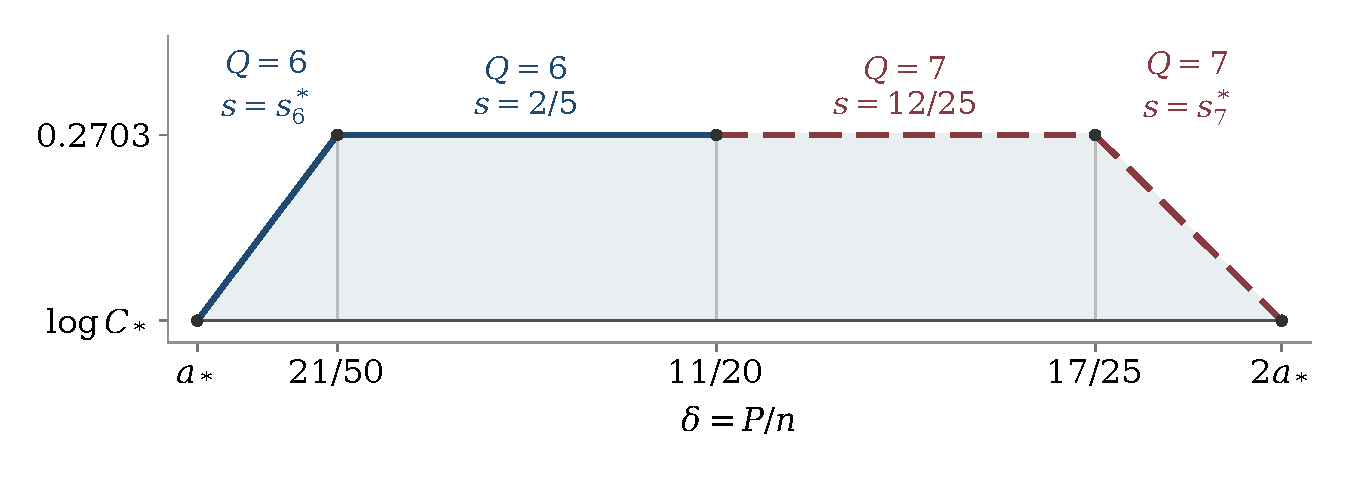
\includegraphics[width=\linewidth]{hoffman-certified-cover.pdf}
\caption{The four chords join proved endpoint lower bounds for the indicated functions $G_Q(\cdot;s)$. Concavity puts each function above its chord, and every chord stays at or above $\log C_*$.}
\label{coverfigure}
\end{figure}

The three interior cutpoints are auxiliary choices; they do not define $C_*$. At the two exterior endpoints the corresponding values equal $\log C_*$. Appendix~\ref{sharp} proves that all six remaining endpoint values exceed $0.2703>\log C_*$. Each concave function lies above the chord joining these endpoint lower bounds, so
\begin{equation}\label{covering}
\begin{split}
\Delta_6(\delta)&\ge\log C_*\quad(a_*\le\delta\le11/20),\\
\Delta_7(\delta)&\ge\log C_*\quad(11/20\le\delta\le2a_*).
\end{split}
\end{equation}
These two coordinate sets suffice for the bound; no claim of optimality among all coordinate sets is needed.

For each sufficiently large $n$, take the least power of two $P\ge a_*n$.
Then $P/n\in[a_*,2a_*)\subset K$. Use $Q=6$ if $P/n\le11/20$ and $Q=7$ otherwise. Combining \eqref{uniform} and \eqref{covering}, and taking the smaller of the two uniform constants, gives
$\chi(\R^n)\ge cC_*^n$. Here the ambient dimension is $n$, as in \eqref{sphere}; setting $n=d$ proves Theorem~\ref{main}.

The need to cover a whole interval disappears if the dimension can be chosen along a sequence. A single rational parameter then gives a stronger base.

\begin{corollary}\label{subsequence}
For infinitely many integers $d$, we have $\chi(\R^d)\ge1.316^d$.
\end{corollary}
\begin{proof}
Put $t_0=131/200$ and $\mu=t_0A_7'(t_0)/A_7(t_0)$. Direct rational substitution gives $1<\mu<1.1$ and
\[
A_7(t_0)>2.03140>1.316\cdot1.54361>1.316E_7(t_0^2).
\]
For $P_\ell=2^\ell$, choose $n_\ell$ to be a nearest integer to $(2P_\ell-1)/\mu$. Then $n_\ell\to\infty$ and $|2P_\ell-1-n_\ell\mu|\le\mu/2<1$. Choose $s=t_0^2$, so that $s^{P_\ell-1}/t_0^{2P_\ell-1}=t_0^{-1}$. Apply Lemma~\ref{coefficients} at $t_0$ to the numerator of \eqref{finitebound}, and its unrestricted upper bound at $s$ to each denominator coefficient. Summing the weights as in \eqref{weighted} gives, for some $c_0>0$ independent of $\ell$ and all sufficiently large $\ell$,
\[
\chi(\R^{n_\ell})\ge
c_0\frac{(1-t_0^2)^2}{t_0}
\left(\frac{A_7(t_0)}{E_7(t_0^2)}\right)^{n_\ell}.
\]
The ratio is strictly greater than $1.316$, so its exponential margin absorbs the constant prefactor for all sufficiently large $\ell$.
\end{proof}

\appendix
\section{Finite rational bounds}\label{arithmetic}
All decimal numbers in this appendix denote exact rational numbers.
We first give the four-row proof of $1.30^d$, then certify the sharper constant. All arithmetic inputs are printed here.

\subsection{Four integer comparisons give \texorpdfstring{$1.30^d$}{1.30\string^d}}\label{rounded}
Take $M=200$, $C=13/10$, and $s=u/M$. For nonnegative integers $c_j$ with $\sum_jc_j=M$ and $\sum_jT_jc_j=2K$, weighted arithmetic--geometric mean gives
\[
A_Q(t)^M\ge\frac{M^M t^{2K}}{\prod_jc_j^{c_j}},\qquad 0^0=1.
\]
Thus, with $G_Q$ as in \eqref{minorant},
\begin{equation}\label{integerwitness}
\begin{split}
G_Q(K/M;u/M)-\log C&\ge M^{-1}\log\mathcal R,\\
\mathcal R&=\frac{M^M(u/M)^K}{C^M E_Q(u/M)^M\prod_jc_j^{c_j}}.
\end{split}
\end{equation}
Table~\ref{roundedtable} lists the inputs and the integer quotients $\lfloor1000\mathcal R\rfloor$, obtained by integer multiplication and division after clearing denominators.

\begin{table}[H]
\centering
\caption{Four integer witnesses with $M=200$.}
\label{roundedtable}
\renewcommand{\arraystretch}{1.15}
\begin{tabular}{c r c r r}
\toprule
$Q$ & $K$ & $(c_0,\ldots,c_{Q-1})$ & $u$ & $\lfloor1000\mathcal R\rfloor$\\\midrule
6 & 75 & $(112,63,21,4,0,0)$ & 75 & 1850\\
6 & 100 & $(100,64,28,7,1,0)$ & 75 & 4288\\
7 & 100 & $(100,64,28,7,1,0,0)$ & 96 & 1288\\
7 & 150 & $(86,62,33,14,4,1,0)$ & 96 & 1391\\\bottomrule
\end{tabular}
\end{table}

Every last-column entry exceeds $1250$, so $\mathcal R>5/4$. Put $\gamma=M^{-1}\log(5/4)>0$. Concavity gives $\Delta_Q(\delta)\ge G_Q(\delta;s)>\log C+\gamma$ on $[3/8,1/2]$ with $(Q,s)=(6,3/8)$, and on $[1/2,3/4]$ with $(Q,s)=(7,12/25)$. Taking the least power of two $P\ge3n/8$ in \eqref{uniform} yields $\chi(\R^n)\ge c_0(C\ee^\gamma)^n\ge1.30^n$ for all sufficiently large $n$. Neither the crossing nor the logarithm enclosures below enter this argument.

\subsection{The sharper constant}\label{sharp}

\paragraph{Logarithms and minimum values.}
For $x>0$, let
\begin{equation}\label{logrule}
\eta=\frac{x-1}{x+1},\qquad
L(x)=2\sum_{j=0}^{15}\frac{\eta^{2j+1}}{2j+1},\qquad
\varepsilon(x)=\frac{2|\eta|^{33}}{33(1-\eta^2)}.
\end{equation}
Then $L(x)-\varepsilon(x)\le\log x\le L(x)+\varepsilon(x)$, by the geometric-series remainder. For accuracy, first write $x=2^k y$ with $1\le y<2$ and use $\log x=k\log2+\log y$, applying \eqref{logrule} to $2$ and $y$. All resulting bounds are rational.

To enclose a minimum, suppose $\mu_b(x_-)<\mu<\mu_b(x_+)$ for $0<x_-<x_+<1$. The function $f(y)=\log Z_b(\ee^y)-\mu y$ is convex, with derivative $f'(y)=\mu_b(\ee^y)-\mu$. Its minimum lies between $\log x_-$ and $\log x_+$. The tangent at the left endpoint therefore gives
\begin{equation}\label{minimumrule}
f(\log x_-)-(\mu-\mu_b(x_-))\log(x_+/x_-)
\le\min_y f(y)\le f(\log x_-).
\end{equation}
Indeed, the tangent has negative slope, so its value at $\log x_+$ is a lower bound throughout that interval.

\paragraph{The crossing.}
Put $N=10^6$. Each row in the next table asserts
\[
k_t/N<t_Q(\delta)<(k_t+1)/N,\qquad
k_s/N<s_Q(\delta)<(k_s+1)/N.
\]
Table~\ref{crossingtable} gives open intervals for $10^9\Delta_Q(\delta)$.

\begin{table}[H]
\centering
\caption{Rational brackets for the crossing.}
\label{crossingtable}
\renewcommand{\arraystretch}{1.2}
\begin{tabular}{c c r r c}
\toprule
$Q$ & $\delta$ & $k_t$ & $k_s$ & $10^9\Delta_Q(\delta)$\\\midrule
6 & $0.371979$ & 562503 & 342209 & $(269455401,269455403)$\\
7 & $0.743958$ & 733755 & 517230 & $(269455447,269455448)$\\
6 & $0.371980$ & 562504 & 342210 & $(269455480,269455481)$\\
7 & $0.743960$ & 733755 & 517231 & $(269455367,269455368)$\\\bottomrule
\end{tabular}
\end{table}

For each $t$ bracket, clear denominators in
$\mu_T(k_t/N)<2\delta<\mu_T((k_t+1)/N)$; for $s$, use $\mu_e$ and $\delta$. Apply \eqref{minimumrule} and \eqref{logrule} to obtain the last column.

The first two rows show $\Delta_6(a_-)<\Delta_7(2a_-)$, and the last two show the reverse inequality at $a_+$. On this bracket, monotonicity of the means gives
\[
t_6<0.563,\quad s_6>0.342,\qquad
t_7(2a)>0.733,\quad s_7(2a)<0.518.
\]
Differentiation at the unique minima gives
$\Delta'_Q(\delta)=\log(s_Q(\delta)/t_Q(\delta)^2)$.
Since $0.342>0.563^2$ and $0.518<0.733^2$, $\Delta_6(a)$ is strictly increasing and $\Delta_7(2a)$ strictly decreasing. This proves existence and uniqueness in \eqref{crossing}. The same log rule yields
\[
\log(1.309251)<\frac{269455219}{10^9},\qquad
\log(1.309252)>\frac{269455900}{10^9}.
\]
Together with the first and third rows, these bounds prove the claimed enclosure for $C_*$ and $\log C_*<0.27$.

\paragraph{The six interior endpoint values.}
For each row below, $k/1000<t_Q(\delta)<(k+1)/1000$, as follows by clearing denominators in the two mean inequalities. Let $L_Q(\delta)$ be the lower bound for $\Phi_Q(2\delta)$ given by \eqref{minimumrule} with these endpoints. For every $s\in[s_-,s_+]$,
\begin{equation}\label{endpointwitness}
G_Q(\delta;s)\ge
L_Q(\delta)-\log E_Q(s_+)+\delta\log s_-.
\end{equation}
Table~\ref{endpointtable} records certified strict lower bounds for the right-hand side, obtained from \eqref{logrule}. For example, its second row uses $t_-=595/1000$, $t_+=596/1000$, $\mu=21/25$ and $s=2/5$ in \eqref{minimumrule} and \eqref{endpointwitness}.

\begin{table}[H]
\centering
\caption{Six interior endpoint bounds. The last column bounds the expression in \eqref{endpointwitness} strictly from below.}
\label{endpointtable}
\renewcommand{\arraystretch}{1.2}
\begin{tabular}{c c r c c c}
\toprule
$Q$ & $\delta$ & $k$ & $s_-$ & $s_+$ & Lower bound\\\midrule
6 & $21/50$ & 595 & $342209/N$ & $342211/N$ & $0.270365$\\
6 & $21/50$ & 595 & $2/5$ & $2/5$ & $0.270573$\\
6 & $11/20$ & 665 & $2/5$ & $2/5$ & $0.270652$\\
7 & $11/20$ & 664 & $12/25$ & $12/25$ & $0.270484$\\
7 & $17/25$ & 714 & $12/25$ & $12/25$ & $0.271274$\\
7 & $17/25$ & 714 & $517230/N$ & $517232/N$ & $0.270342$\\\bottomrule
\end{tabular}
\end{table}

The crossing brackets and monotonicity imply that $s_6^*$ and $s_7^*$ lie in the intervals in the first and last rows. Since $0.2703>0.27>\log C_*$, this proves all six strict inequalities used in Section~\ref{coversection}.

\paragraph{Acknowledgement.}
AI-assisted tools were used in mathematical exploration, exact-arithmetic verification, and preparation of this manuscript. This assistance included the spherical-layer construction and detector-index remark in Section~\ref{geometry}, the counting argument in Section~\ref{counting}, and the concave covering and subsequential bound in Section~\ref{coversection}.

\begin{thebibliography}{9}
\bibitem{fw} P. Frankl and R. M. Wilson, Intersection theorems with geometric consequences, \emph{Combinatorica} \textbf{1} (1981), 357--368. \href{https://doi.org/10.1007/BF02579457}{doi:10.1007/BF02579457}.
\bibitem{convex} E. S. Gorskaya, I. M. Mitricheva, V. Yu. Protasov, and A. M. Raigorodskii, Estimating the chromatic numbers of Euclidean space by convex minimization methods, \emph{Sb. Math.} \textbf{200} (2009), 783--801. \href{https://doi.org/10.1070/SM2009v200n06ABEH004019}{doi:10.1070/SM2009v200n06ABEH004019}.
\bibitem{kula} A. Kula, M. Omar, J. Stockwell, and M. Xie, Multiple distance Ramsey bounds for graphs in Euclidean spaces, preprint (2026), \href{https://arxiv.org/abs/2608.05860}{arXiv:2608.05860}.
\bibitem{kuznetsov} A. Kuznetsov, Using $q$-calculus to study $LDL^T$ factorization of a certain Vandermonde matrix, \emph{Operators and Matrices} \textbf{12} (2018), 773--777. \href{https://doi.org/10.7153/oam-2018-12-45}{doi:10.7153/oam-2018-12-45}.
\bibitem{naslund} E. Naslund, The chromatic number of $\R^n$ with multiple forbidden distances, \emph{Mathematika} \textbf{69} (2023), 692--718. \href{https://doi.org/10.1112/mtk.12197}{doi:10.1112/mtk.12197}.
\bibitem{rai} A. M. Raigorodskii, On the chromatic number of a space, \emph{Russian Math. Surveys} \textbf{55} (2000), 351--352. \href{https://doi.org/10.1070/RM2000v055n02ABEH000281}{doi:10.1070/RM2000v055n02ABEH000281}.
\bibitem{survey} A. M. Raigorodskii and P. S. Sinelnikov-Murylev, Johnson graphs, their random subgraphs, and some of their extremal characteristics, \emph{Russian Math. Surveys} \textbf{80} (2025), 471--530. \href{https://doi.org/10.4213/rm10233e}{doi:10.4213/rm10233e}.
\end{thebibliography}
\end{document}
